\section{Konzept} % Daniel
\begin{frame}
    \frametitle{Konzept}
    \begin{columns}
        \begin{column}{0.4\textwidth}
            \begin{block}{Teilkonzepte}
                \begin{itemize}
                    \item<2-> Korberkennung
                    \item<3-> Ausrichtung
                    \item<4-> Ballbeschleunigung
                    \item<5-> Ballnachführung
                    \item<6-> Kommunikation
                    \item<7-> Energieversorgung
                \end{itemize}
            \end{block}
        \end{column}
        \begin{column}{0.6\textwidth}
            \centering
            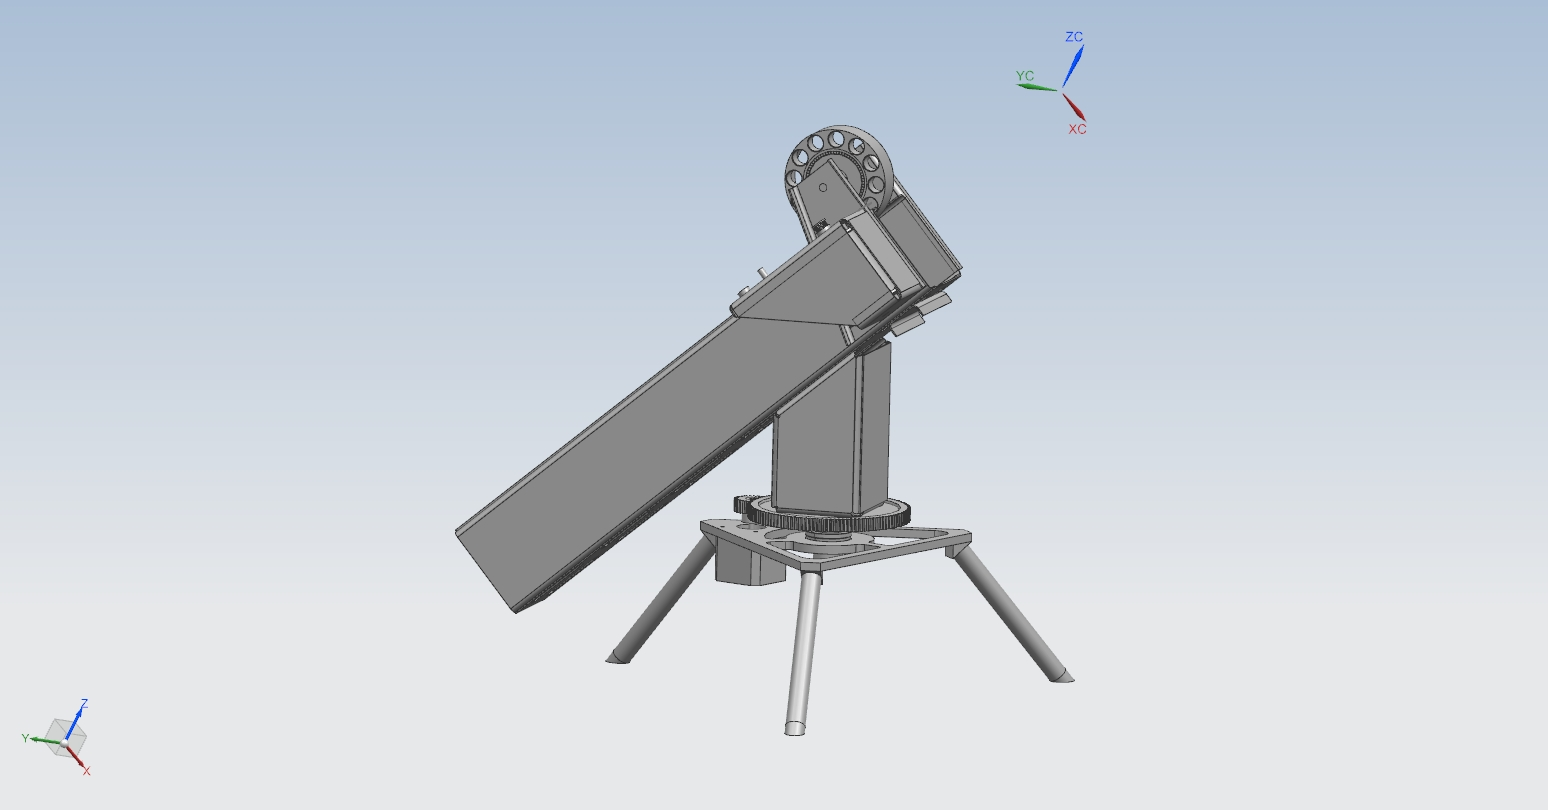
\includegraphics[width=0.8\textwidth, trim = 150mm 50 150mm 10, clip]{../doc/fig/Gesamt_bg1.jpg}
        \end{column}
    \end{columns}
\end{frame}

\begin{frame}
    \frametitle{Konzept}
    \framesubtitle{Korberkennung}
    \begin{columns}
        \begin{column}{0.4\textwidth}
            \begin{block}{Korberkennung}
                \begin{itemize}
                    \item Kamera
                    \item OpenCV
                \end{itemize}
            \end{block}
        \end{column}
        \begin{column}{0.6\textwidth}
        \end{column}
    \end{columns}
\end{frame}


\begin{frame}
    \frametitle{Konzept}
    \framesubtitle{Korberkennung --- Sensoren}
    \begin{columns}
        \pause
        \begin{column}{0.5\textwidth}
            \begin{block}{Ultraschall - HC-SR04}
                \begin{itemize}
                    \item Laufzeit Ultraschallimpuls
                    \item $D = \frac{T \cdot c_{Luft}}{2}$
                \end{itemize}
                \pause
                \begin{figure}
                    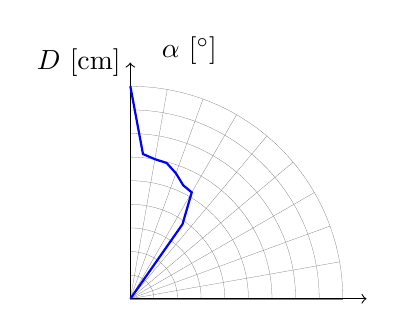
\begin{tikzpicture}[scale=1.5]
                        % Grid
                        % Grid for Angle
                        \foreach \i in {0, 10, ..., 90}
                        {
                            \draw[ultra thin, gray]
                                (90-\i:0) -- (90-\i:1.8);
                                %node[above right, black] {\i};
                        }
                        % Grid for Distance
                        \foreach \i in {0, 20, ..., 180}
                        {
                            \draw[ultra thin, gray]
                                (0.01*\i,0) arc [radius = 0.01*\i, start angle = 0, end angle = 90];
                                %node[left, black] {\i};
                        }
                        % Axis
                        \draw[->] (0:0) -- (0:2);
                        \draw[->] (0:0) -- (90:2) node[left] {$D$ [cm]};
                        \node at (0.5, 2.1) {$\alpha$ [$^\circ$]};
                        % Data
                        \draw[thick, blue]
                            (90 - 0  : 1.80) --
                            (90 - 5  : 1.23) --
                            (90 - 10 : 1.20) --
                            (90 - 15 : 1.19) --
                            (90 - 20 : 1.13) --
                            (90 - 25 : 1.06) --
                            (90 - 30 : 1.04) --
                            (90 - 35 : 0.77) --
                            (90 - 40 : 0.00) ;
                    \end{tikzpicture}
                \end{figure}
            \end{block}
        \end{column}
        \pause
        \begin{column}{0.5\textwidth}
            \begin{block}{Infrarot - GP2Y0A710K0F}
                \begin{itemize}
                    \item Triangulation
                    \item $D = d \cdot \arctan(\alpha)$
                \end{itemize}
                \pause
                \begin{figure}
                    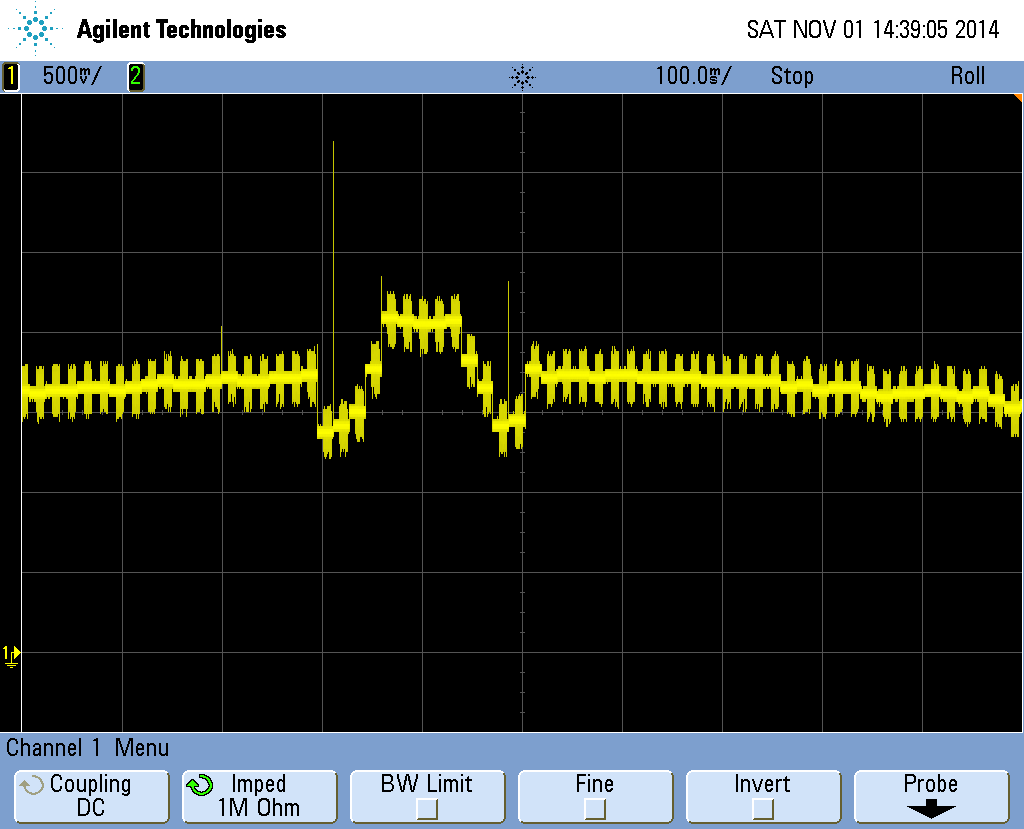
\includegraphics[width=0.8\textwidth]{../doc/fig/scope_80.png}
                \end{figure}
            \end{block}
        \end{column}
    \end{columns}
\end{frame}



\begin{frame}
    \frametitle{Konzept}
    \framesubtitle{Ausrichtung}
    \begin{columns}
        \begin{column}{0.4\textwidth}
            \begin{block}{Ausrichtung}
                \begin{itemize}
                    \item Drehung
                    \item Getriebe
                    \item Schrittmotor
                \end{itemize}
            \end{block}
        \end{column}
        \begin{column}{0.6\textwidth}
            \centering
            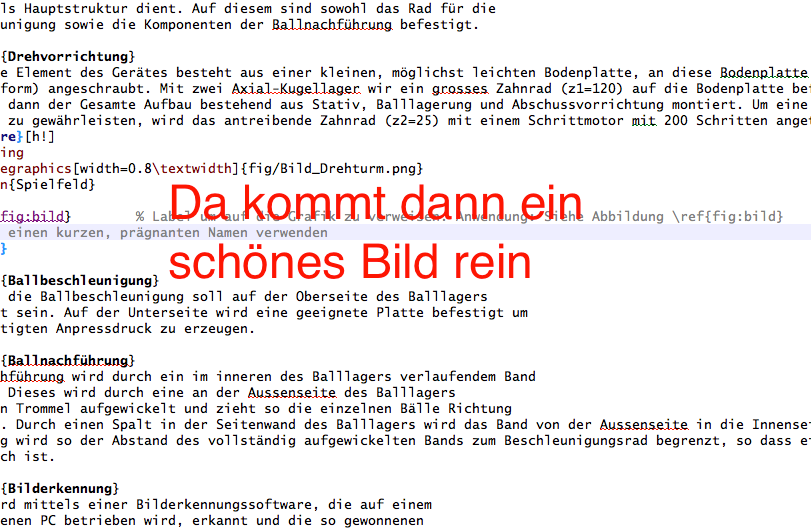
\includegraphics[width=1.0\textwidth, trim = 25mm 23mm 5mm 15mm, clip]{../doc/fig/Bild_Drehturm.png}
        \end{column}
    \end{columns}
\end{frame}



\begin{frame}
    \frametitle{Konzept}
    \framesubtitle{Ballbeschleunigung}
    \begin{columns}
        \begin{column}{0.4\textwidth}
            \begin{block}{Ballbeschleunigung}
                \begin{itemize}
                    \item Ein Rad oberhalb
                    \item<2-> BLDC Motor
                \end{itemize}
            \end{block}
            \centering
            \pause
            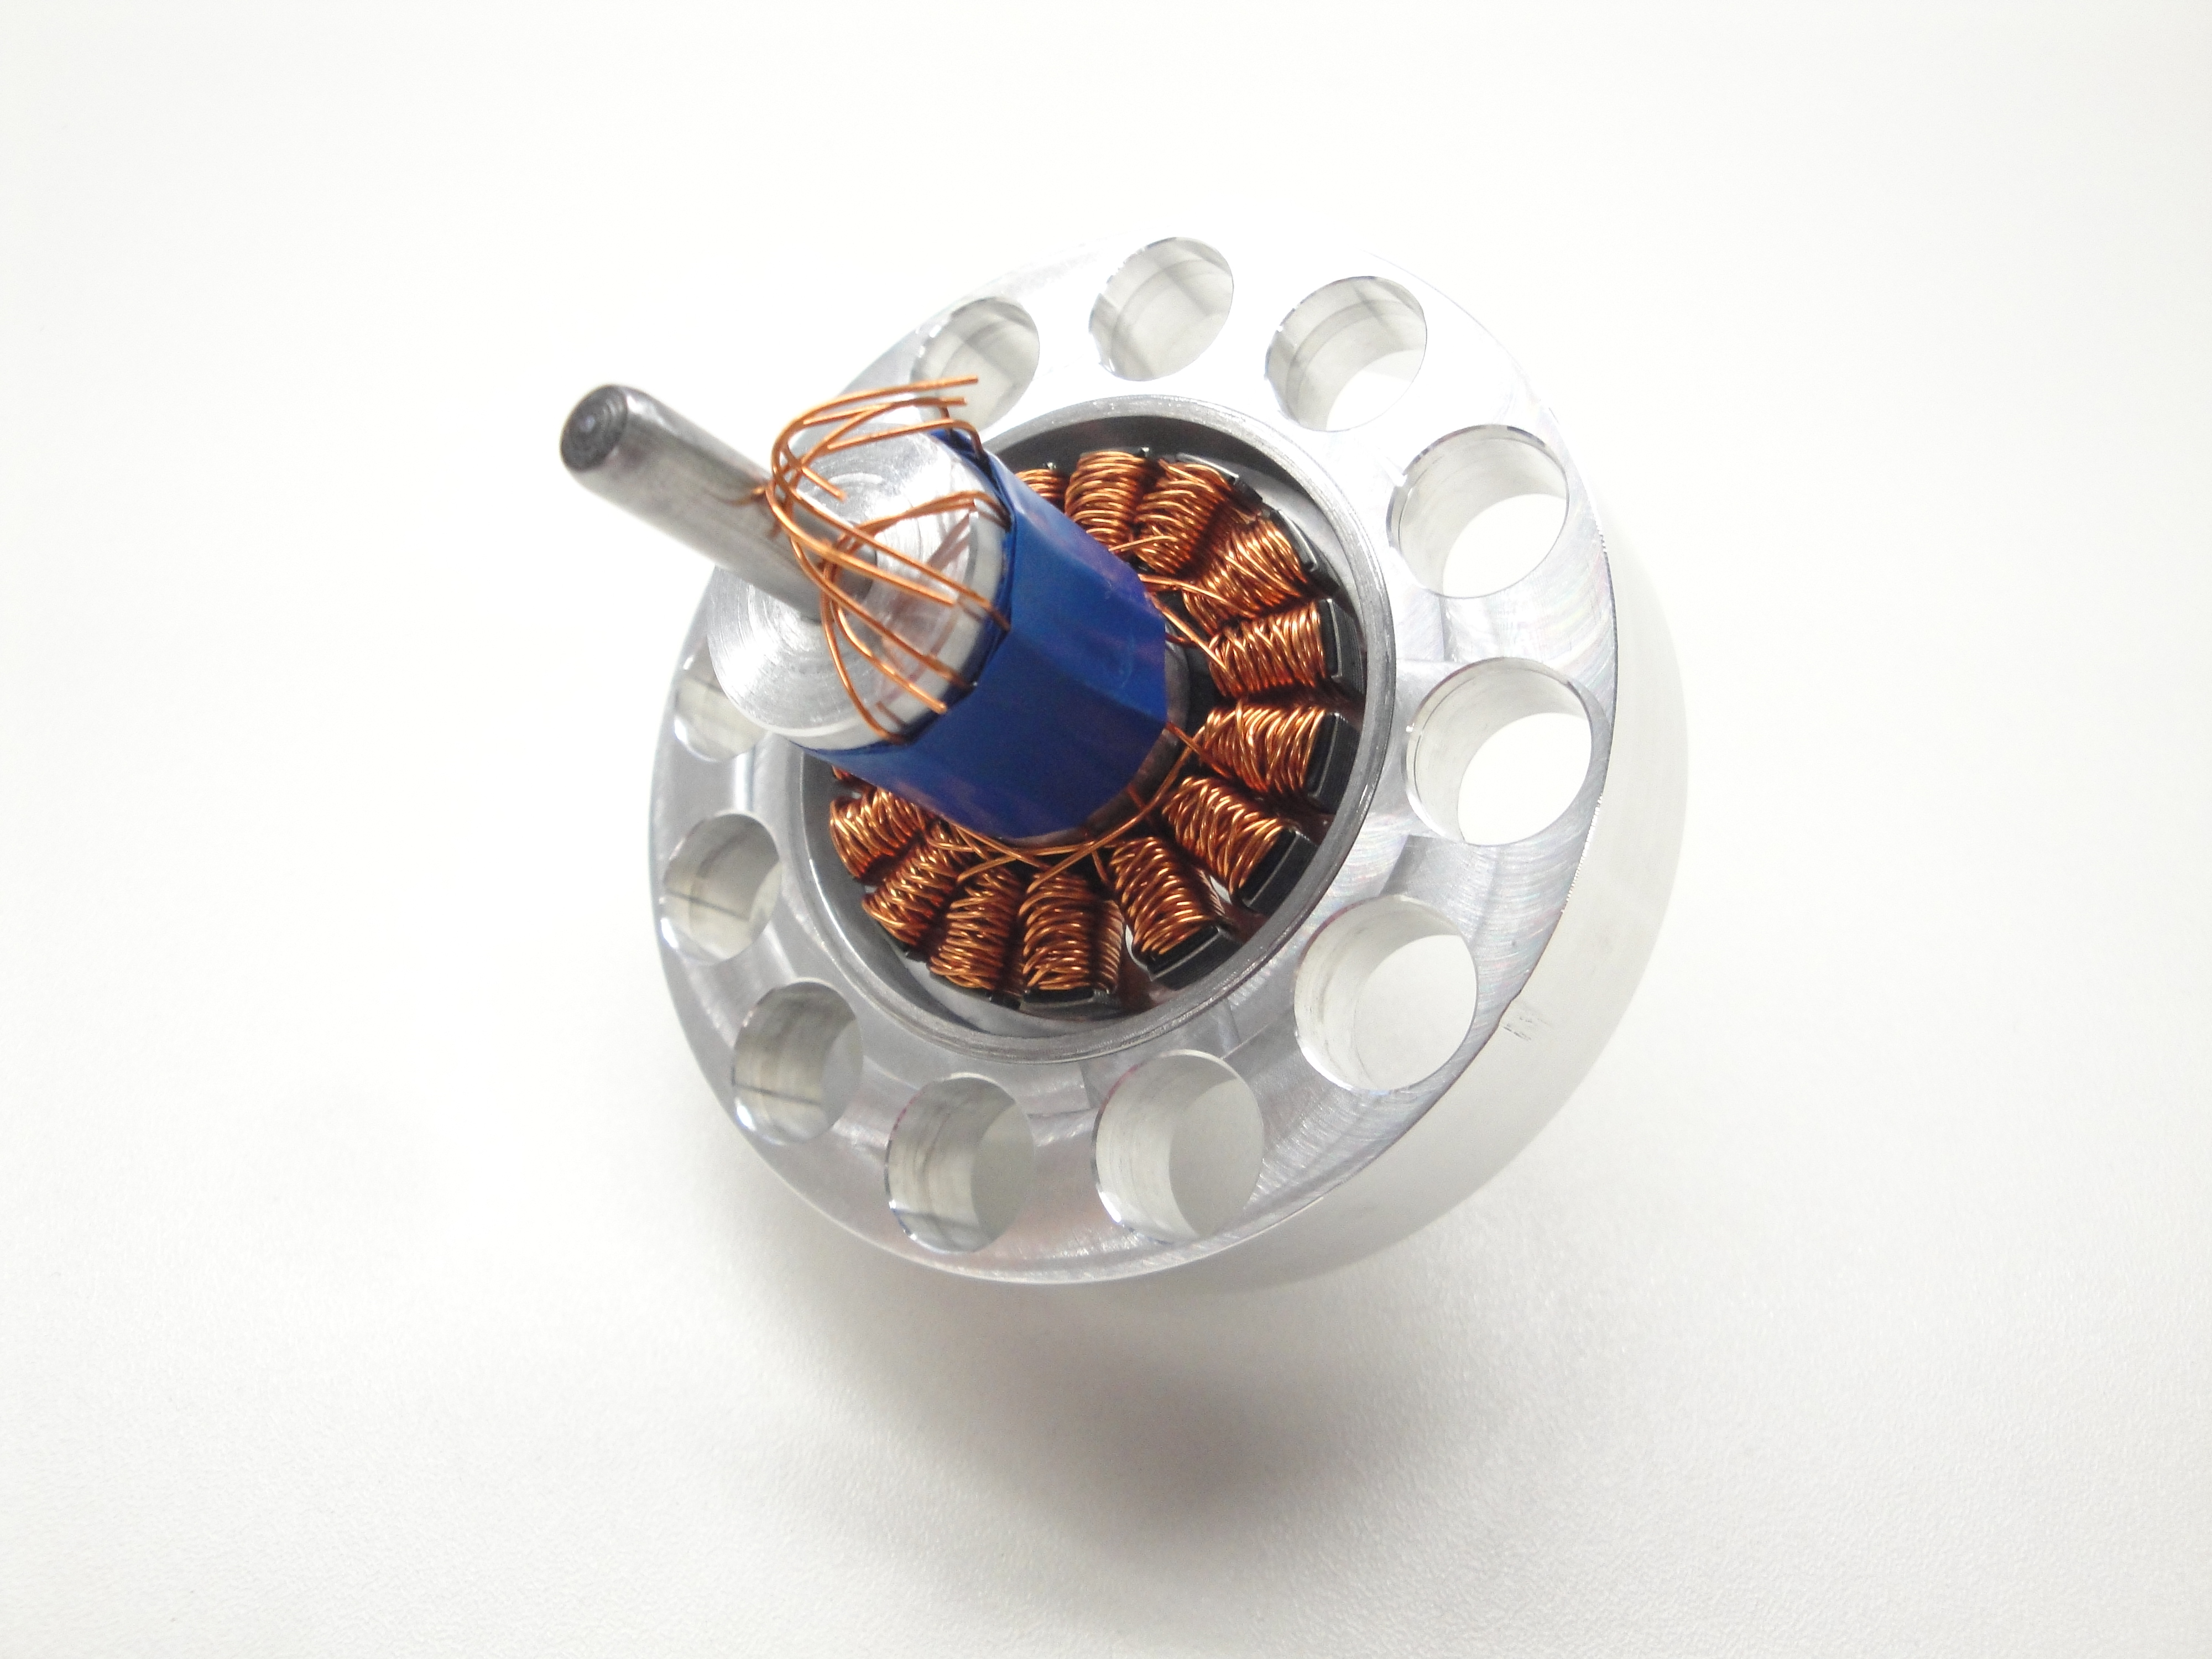
\includegraphics[width=0.8\textwidth, trim = 330mm 200mm 300mm 100mm, clip]{../fig/bldc/DSC02754.JPG}
        \end{column}
        \begin{column}{0.6\textwidth}
            \centering
            \onslide
            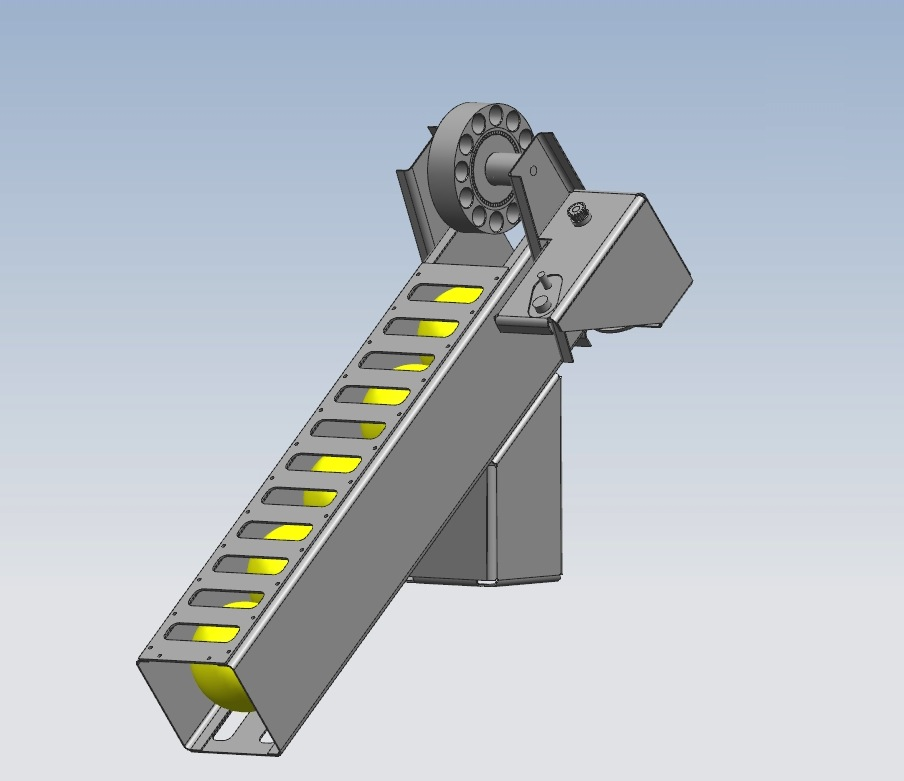
\includegraphics[width=0.8\textwidth, trim = 40mm 0mm 60mm 30mm, clip]{../doc/fig/Balllager.jpg}
        \end{column}
    \end{columns}
\end{frame}


\begin{frame}
    \frametitle{Konzept}
    \framesubtitle{Ballbeschleunigung --- Ballwurf}
    \begin{figure}[h!]
        \centering
        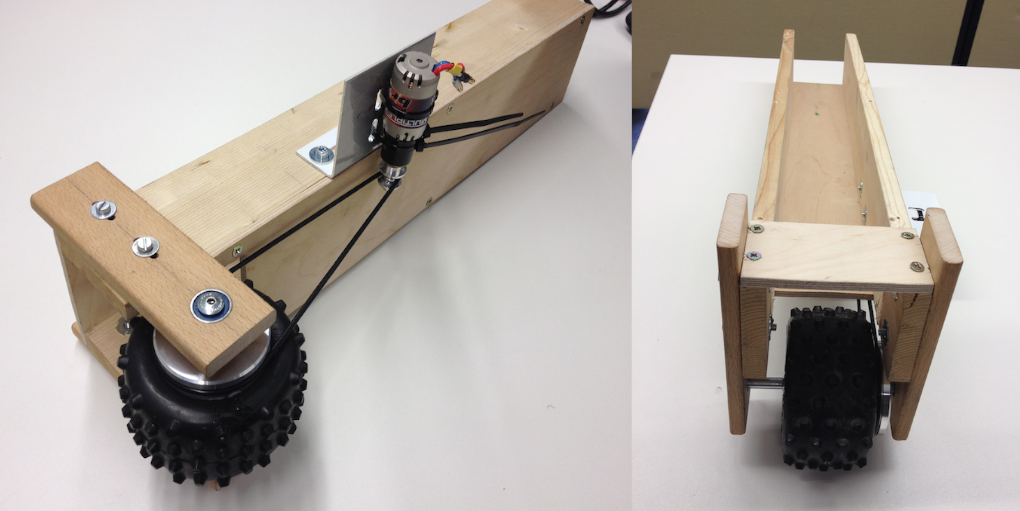
\includegraphics[width=0.6\textwidth]{../doc/fig/Schussvorrichtung.png}
        \caption{Versuchsaufbau Ballwurf}
    \end{figure}
\end{frame}


\subsection{BLDC Ansteuerung}
    Diese Messung wird gemeinsam mit Gruppe 32 durchgeführt. \\

\subsubsection{Aufbaubeschreibung}
    \begin{figure}[h!]
       	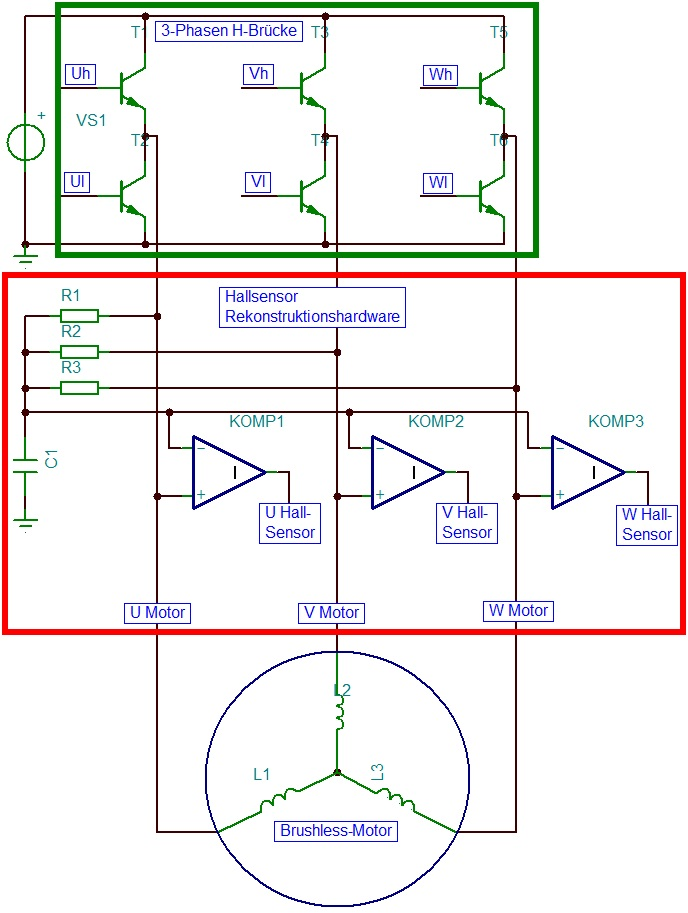
\includegraphics[scale=0.60]{fig/MotoransteuerungSchema.jpg}
       	\centering
       	\caption{Schema des Brushless-Versuchsaufbaus}
        \label{abb:MotoransteuerungSchema}
    \end{figure}
    \noindent Das Schema des Gesamtaufbaus des Tests ist in der Abbildung 
    \ref{abb:MotoransteuerungSchema} ersichtlich. Die 3-Phasen H-Brücke im 
    oberen grünen Rechteck wird direkt vom FPGA\footnote
    {\textbf{F}ield-\textbf{P}rogrammable \textbf{G}ate 
    \textbf{A}rray} angesteuert. Die Hardware dieser Brücke ermöglicht eine 
    voll galvanisch getrennte Ansteuerung mit $3.3 V$ Logikpegeln. Diese 
    Brücke wurde zur Verfügung gestellt und direkt verwendet. Die 
    Rekonstruktion der Hallsensoren-Signale findet im rot markierten Teil des 
    Aufbaus statt. Dieser Part wird auf einer Laborplatte aufgebaut und 
    gelötet. Die so generierten Signale $U_{Hallsensor}$, $V_{Hallsensor}$, 
    $W_{Hallsensor}$ werden einem FPGA geliefert. Anhand dieser Signale 
    steuert das FPGA die H-Brücken-Transistoren mit den Signalen $U_h$, $U_l$, 
    $V_h$, $V_l$, $W_h$, $W_l$. Die im FPGA enthaltene Konfiguration besteht 
    aus simplen AND-Verknüpfungen, die die anliegenden Signale sehr schnell 
    und effizient verarbeiten können. Auf diese Weise ist es möglich, den 
    Motor sehr schnell anzusteuern.
    In der Abbildung \ref{abb:MessplatzAufbau} ist der gesamte Aufbau 
    abgebildet. Man beachte die markierten Felder. Am linken unteren Rand ist 
    der Motor befestigt. In der Mitte des Bildes ist die Hardware zur 
    Rekonstruktion der Hallsensoren-Signale.  Die generierten Signale werden 
    dem FPGA in der unteren rechten Ecke zugeführt. Diese Signale werden 
    logisch verknüpft und danach die sechs Signale generiert, um die H-Brücke 
    in der rechten oberen Hälfte anzusteuern.  Die H-Brücken wiederum treiben 
    den Motor an.
    \begin{figure}[h!]
    %\vspace{-16pt}
       	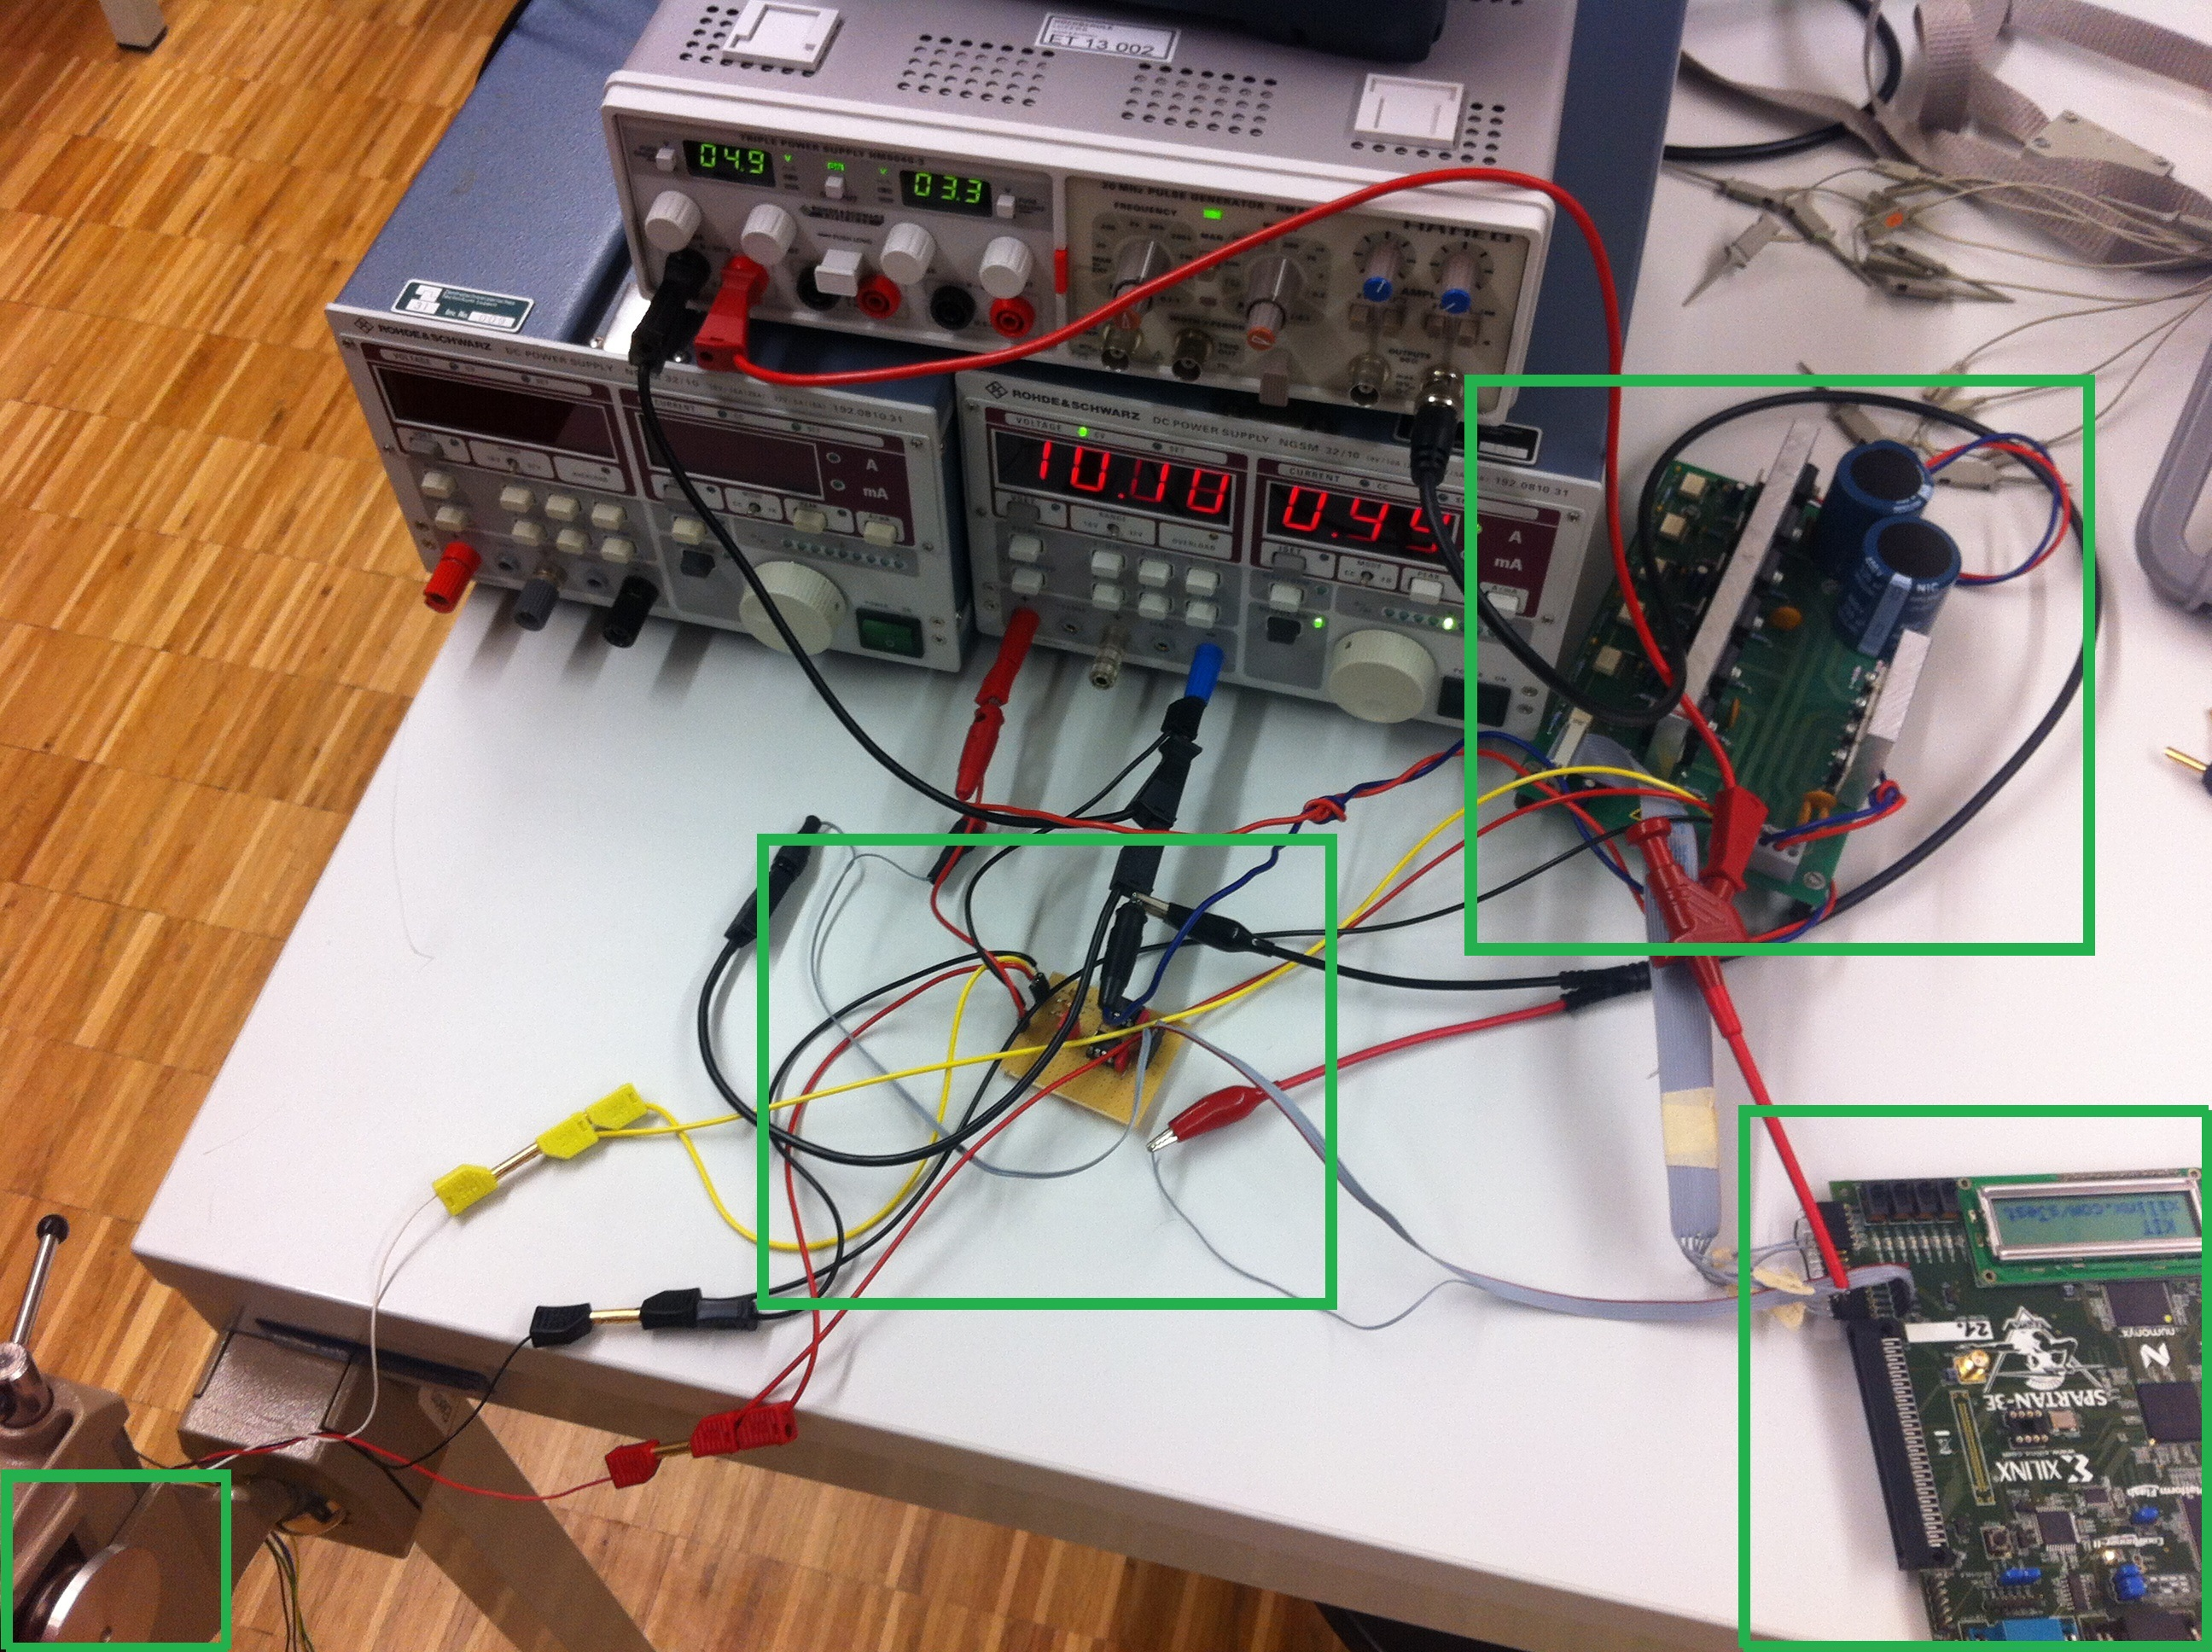
\includegraphics[width=0.9\textwidth]{fig/MessplatzAufbau.jpg}
       	\centering
       	\caption[Testaufbau BLDC Treiber]{Testaufbau} 
        \label{abb:MessplatzAufbau}
    %\vspace{-10pt}
    \end{figure}
    Die im FPGA enthaltene Logik basiert auf der Wahrheitstabelle, die in 
    Tabelle \ref{abb:WahrheitstabelleAnsteuerung} abgebildet ist.
    \begin{table}[h!]
        \begin{zebratabular}{ccc||cc|cc|cc||c}
             \rowcolor{gray}
             $H_1$ & $H_2$ & $H_3$ & $U_h$ & $U_l$ & $V_h$ & $V_l$ & $W_h$ & $W_l$ & Illegal\\
               0   &   0   &   0   &   0   &   0   &   0   &   0   &   0   &   0   &   1\\
               0   &   0   &   1   &   0   &   0   &   0   &   1   &   1   &   0   &   0\\
               0   &   1   &   0   &   0   &   1   &   1   &   0   &   0   &   0   &   0\\
               0   &   1   &   1   &   0   &   1   &   0   &   0   &   1   &   0   &   0\\
               1   &   0   &   0   &   1   &   0   &   0   &   0   &   0   &   1   &   0\\
               1   &   0   &   1   &   1   &   0   &   0   &   1   &   0   &   0   &   0\\
               1   &   1   &   0   &   0   &   0   &   1   &   0   &   0   &   1   &   0\\
               1   &   1   &   1   &   0   &   0   &   0   &   0   &   0   &   0   &   1\\
        \end{zebratabular}
        \centering
        \caption[Wahrheitstabelle der Ansteuerung für den BLDC Treiber]{Wahrheitstabelle der Ansteuerung}
        \label{abb:WahrheitstabelleAnsteuerung}
    \end{table}

\clearpage
\subsubsection{Messmittel}
    \begin{table}[h!]
        \centering
        \begin{zebratabular}{lll}
            \rowcolor{gray}
            Gerät &
                Typ &
                Nummer \\
            Speisegerät & 
                Rohde \& Schwarz NGSM 32/10 &
                Inv.-Nr. 009 \\
            Oszilloskop &
                Agilent MSO6052A &
                Inv.-Nr. 48; S/N: MY44001903 \\
            Mainframe &
                Hameg HM8001-2 &
                SN: 059520046 \\
            Speisegerät &
                Hameg HM8040-3 &
                SN: 015405014 \\
            Pulsgenerator &
                Hameg HM8035 &
                Inv.-Nr. 44 \\
        \end{zebratabular}
        \caption[Messmittel des Versuchsaufbaus für den BLDC Treiber]{Messmittel des Versuchsaufbaus}
    \end{table}

\subsubsection{Resultat}
\label{chap:VersuchsResultat}
Mit dem beschriebenen Aufbau konnte ein BLDC-Motor erfolgreich angesteuert 
werden. Wie in Abbildung \ref{abb:MessplatzAufbau} am linken unteren Rand zu 
erkennen ist, ist an der Motorwelle eine Aluminiumplatte montiert. Mit dieser 
und einem Magneten konnte der Motor mittels einer Wirbelstrombremse belastet 
werden. Auf diese Weise konnte rund $120 W$ elektrische Leistung umgesetzt 
werden. Dabei stellte sich heraus, dass die PWM nachgeregelt werden muss, wenn 
eine Last getrieben wird. Weiter bietet der Aufbau, so wie er getestet wurde, 
keine Möglichkeit den Motor ohne äussere Manipulation zu starten.\\
\\
Diese beiden Tatsachen sprechen dafür, dass das Prinzip grundsätzlich 
funktioniert. Für die Realisierung würde sich ein eigenes Board anbieten, auf 
dem ein eigener Controller die Regelung und die Zwangskommutierung beim 
Starten des Motors übernimmt.


\begin{frame}
	\frametitle{Konzept}
	\framesubtitle{Ballnachführung}
	\begin{columns}
		\begin{column}{0.4\textwidth}
			\begin{block}{Ballbeschleunigung}
				\begin{itemize}
					\item Stahlband
					\item DC Motor
				\end{itemize}
			\end{block}
			\centering
			\rule{0pt}{0.8\textwidth}
		\end{column}
		\begin{column}{0.6\textwidth}
			\centering
			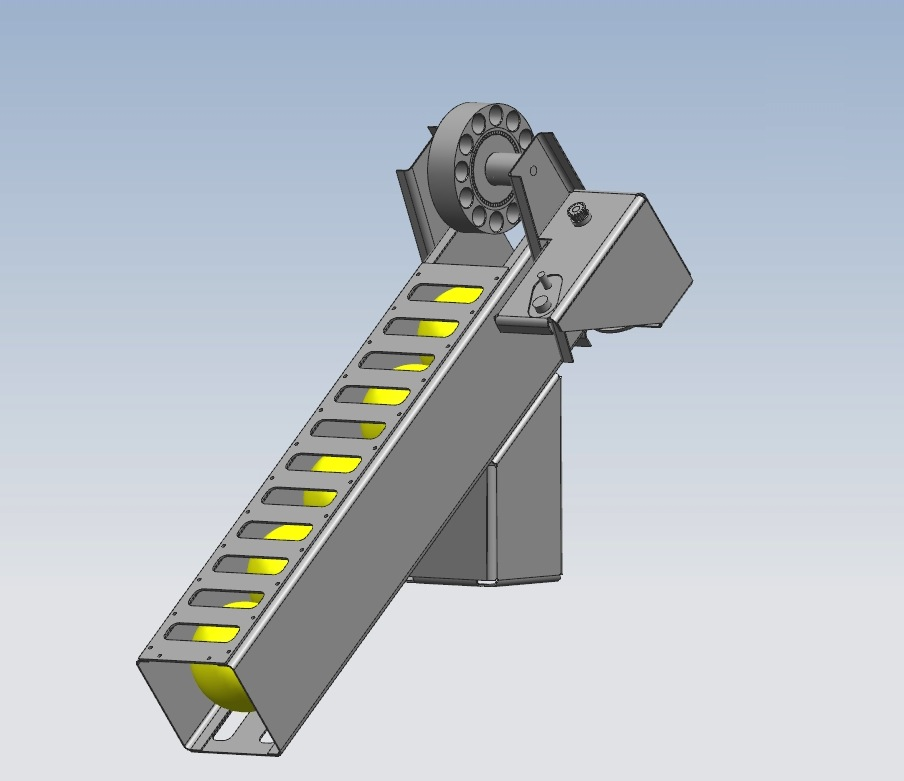
\includegraphics[height=0.8\textwidth, trim = 40mm 0mm 60mm 30mm, clip]{../doc/fig/Balllager.jpg}
		\end{column}
	\end{columns}
\end{frame}

\begin{frame}
    \frametitle{Konzept}
    \framesubtitle{Kommunikation}
    \begin{columns}
        \begin{column}{0.4\textwidth}
            \begin{block}{Kommunikation}
                \begin{itemize}
                    \item WLAN für Kamerabild
                    \item Bluetooth für Steuerung
                \end{itemize}
            \end{block}
        \end{column}
        \begin{column}{0.6\textwidth}
            \centering
            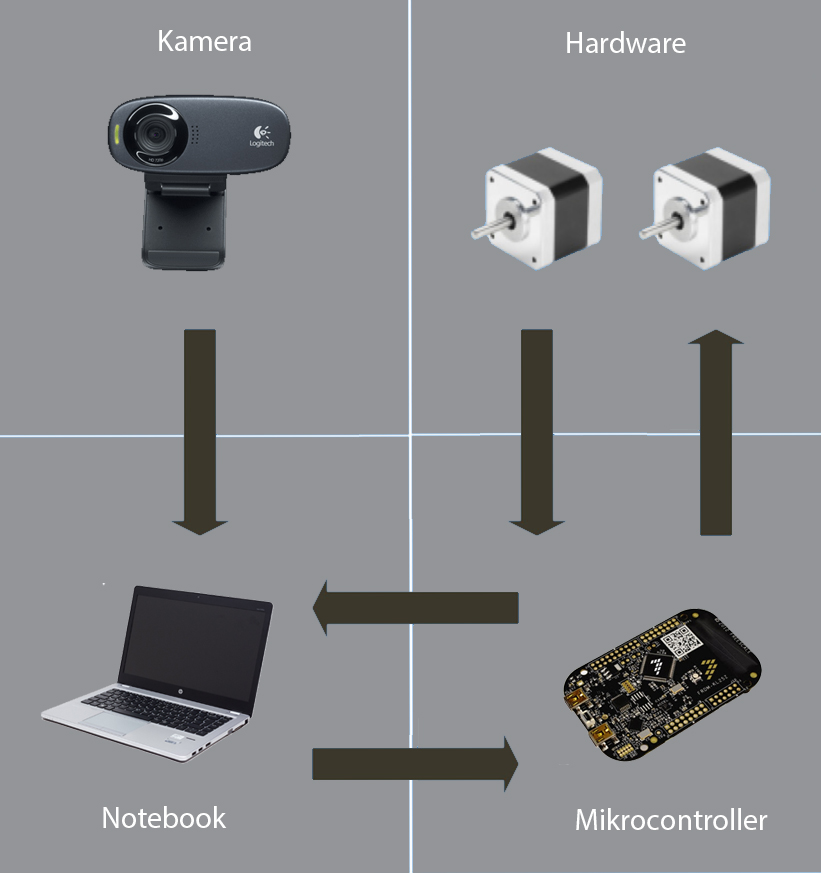
\includegraphics[width=0.7\textwidth]{../doc/fig/kommunikationsablauf.jpg}
        \end{column}
    \end{columns}
\end{frame}



\begin{frame}
    \frametitle{Konzept}
    \framesubtitle{Energieversorgung}
    \begin{block}{Energieversorgung}
        \begin{itemize}
            \item Netzteil
            \item 24 \ldots 36 V
        \end{itemize}
    \end{block}
\end{frame}


